\chapter{ReLUSyn}
\label{relusyn}
In this section we explain the inner workings of our tool ReLUSyn. 
There are two parts to this; we first explain our approach and our algorithms that are used for the synthesis, and we then talk about our tool \tool that implements the algorithms and synthesizes the models and attacks. 
We show how fully connected feed-forward \ac{DNN}s can be formulated as \ac{MILP} models. 
We use a generic representation and describe the modeling of cost functions that are used to generate \ac{RFDIA}.
We then show how this allows us to identify critical inputs and find the perturbations. 
We finally explain how we map this to real systems.
We also include a section on how ReLU (the non-linear activation function) might be modeled internally by MILP solvers based on work by Fischetti et al. \cite{fischetti2017deep}, where they propose a 0-1 MILP model for DNN modeling.
This section is included for completeness as the solver we use for our evaluation is able to handle the $\max$ function automatically.

\begin{figure}
	\centering
	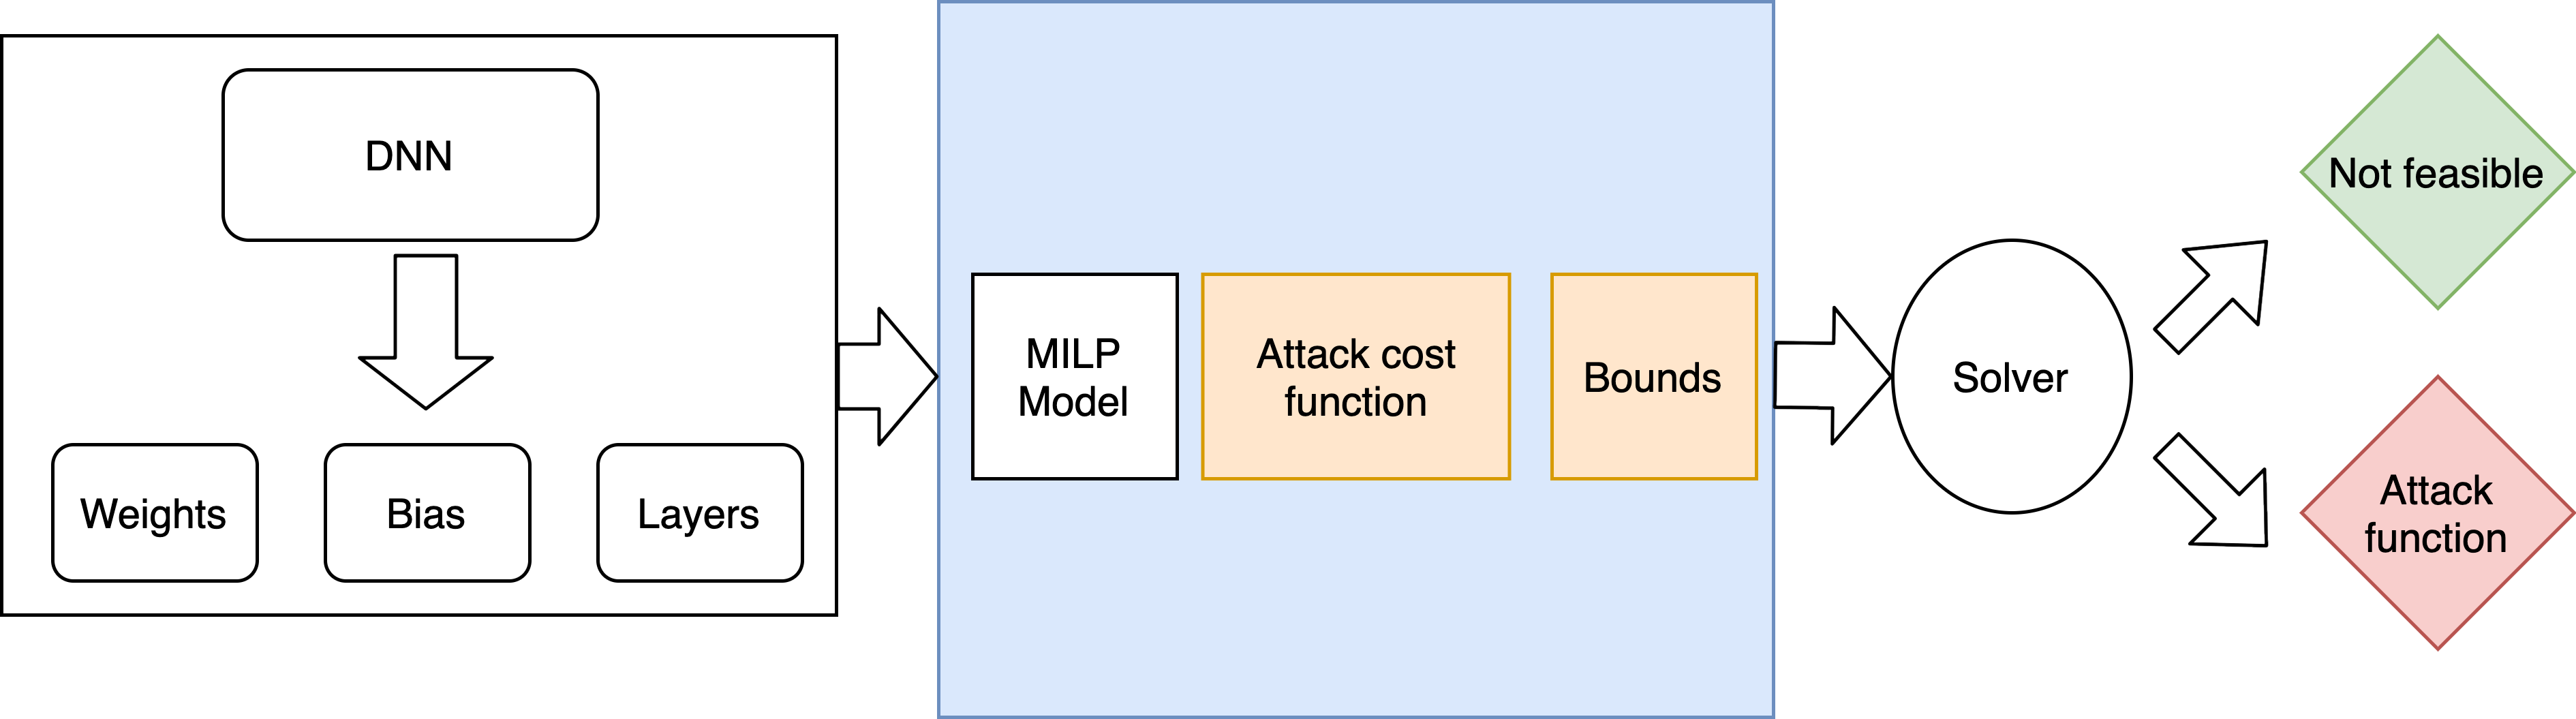
\includegraphics[scale=0.1]{Images/Methodology}
	\caption[Methodology]{The rounded boxes depict the information provided by the users and the sharp corners is the information provided by us that integrates the first layer into the solver layer.}
	\label{fig:methodology}
\end{figure}

\begin{figure}
	\centering
	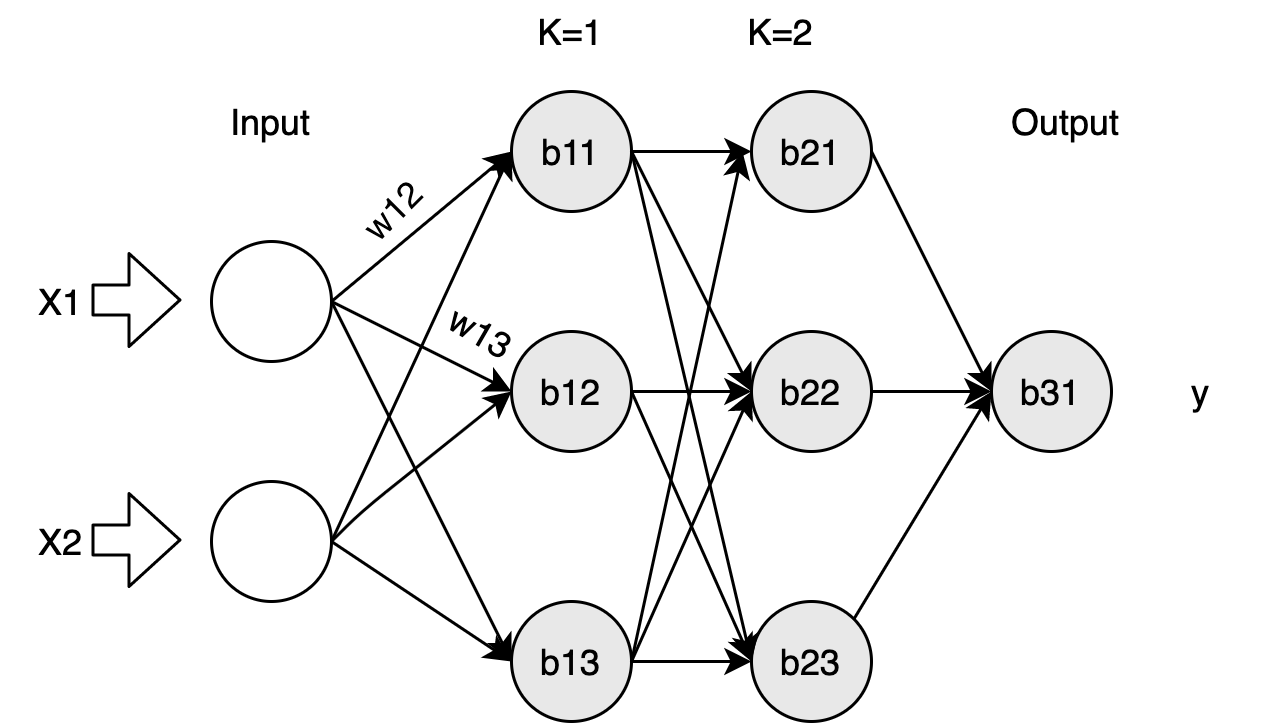
\includegraphics[width=0.7\linewidth]{Images/DNNstructure}
	\caption[DNN structure]{DNN controller structure with two hidden layers K=1,2, two inputs x1 and x2 and one output y. This is an example of a fully connected network.}
	\label{fig:dnn-controller}
\end{figure}


\section{ReLUSyn: Overview}
ReLUSyn is the tool that models our approach, and allows the attacker to generate \ac{RFDIA} attacks directly from the \ac{DNN} model. 
Our technique is shown in Figure ~\ref{fig:methodology}.
The \ac{DNN} is made available from the systems which can be directly passed through \tool. 
It automatically synthesizes a \ac{MILP} model from the \ac{DNN} model which also contains the input value bounds.
The attacker can specify a cost function if they possess the relevant domain-specific knowledge to make such a decision. 
The cost function determines the kind of attack to be launched on the system.
Everything inside the blue box is automatically synthesized in Figure ~\ref{fig:methodology}.
The cost function and bounds have a plug-gable functionality. 
Everything inside the blue box is automatically synthesized.
The orange parts can be easily changed to extend the technique for different systems and applications in the future. 
The models along with the cost functions and bounds are passed through a MILP solver; the solver finds an optimal solution for the MILP model, and this optimal solution corresponds to an attack. If the solver determines the model is infeasible, then no attacks exist.
Each feasible solution of the model corresponds to a particular attack and the optimal solution corresponds to the preferred attack as specified by the user's cost function. We discuss the concept of using cost functions to launch specific attacks later in this chapter.
	
\section{DNN formalism}
We follow the formalism based on the general architecture that we explain in Chapter ~\ref{background}. 
The \ac{DNN} controller maps the inputs that are the $x1$ and $x2$ to the output $y$ as shown in  Figure ~\ref{fig:dnn-controller}.   
We now begin with the formal modeling of the \ac{DNN}.


%Formal modeling of a DNN for later use when explaining the modeling in MILP  
The architecture can be represented as a function F defined as $F: X \rightarrow Y$ where the inputs X are mapped to the output Y and are composed of multiple layers. 
We consider \ac{DNN} to be made up of $K + 1$ layers, numbered from 0 to K.
Layer 0 %does not really exist since it 
is the input layer of the network, while
the last layer K corresponds to the output of the \ac{DNN}.
Every individual layer in the \ac{DNN} $k$ $\epsilon$ $\{0,1,....,K\}$ consists of $n_k$ nodes or neurons in the network.
Each neuron has a bias associated with it. 
Every neuron from the previous layer is connected to every neuron in the next layer. 
The neurons are labeled starting from $1$ to $n_k$ in the network. 
We denote every neuron by $NODE(i,k)$ which corresponds to the $ith$ node for the layer k. 

We denote the output vector of the layer $k$ as $F_k(x)$.
The output for every $NODE(i,k)$ denoted as $F_{ik}(x)$ where $i$ $\epsilon$ $\{0,1,....,n_k\}$ 

The output for layer 0 is represented as $F_k(0)$.
For every layer $k \geq 1$ the output vector is represented in Equation ~\ref{1}. 

\begin{equation}
\label{1}
\begin{aligned}
F_k(x) &= \upsigma(W^{k-1}x^{k-1} + b^{k-1}) \\
\end{aligned}
\end{equation}

where $\upsigma$ represents the activation function being used in the DNN under consideration. 
There are multiple types of activation functions with different modeling capabilities, such as ReLU ($f(x) = max {0,x}$) as shown in Figure 	\ref{fig:relubreakdown} and logistic (or sigmoid) activation function $f(x)=1/(1+ exp(-e))$.
\tool focuses on using Rectified Linear Unit (ReLU) since it is one of the commonly used activation functions in \ac{DNN}s as Krizhevsky et al. \cite{10.1145/3065386}. 
Hence, our equation now looks something like where, for a vector $x$, \texttt{ReLU}($x$):= $\sum_{i=1}^{n} e_{i}\max(0, x_{i})$ (per layer).



\begin{equation}
\label{2}
\begin{aligned}
F_k(x) &= ReLU(W^{k-1}x^{k-1} + b^{k-1}) \\
\end{aligned}
\end{equation}

Since a network consists of multiple layers, the general \ac{DNN} representation looks like a composition function as shown below. 
\begin{equation}
\label{3}
	\begin{aligned}
	F(x) &= F_K \circ F_{K-1} \circ F_{K-2} ....... \circ F_1(x),    \\
	or \\
	F(x) &= F_K ( F_{K-1}( F_{K-2} .......  (F_1(x)))),    \\
	\end{aligned}
\end{equation}

%This ends  our \ac{DNN} formalism. In the next section we use the formalism to create a \ac{MILP} model. 

\section{MILP Model}
The ReLU activation function cannot be modeled directly by MILP solvers. 
This section presents an
equivalent formulation that is accepted by such solvers which we use to locate critical inputs and find the minimum perturbations as explained in ~\ref{problemstatement}. 
The solver we use Gurobi handles this conversion
internally without exposing the user to the details. 
We have decided to include it here for the purpose of completeness.

 
To create a \ac{MILP} model, the essence lies in studying the basic scalar equation that describes the \ac{DNN} architecture. 

\begin{equation}
\label{4}
\begin{aligned}
x &= ReLU(w^Ty + b) \\
\end{aligned}
\end{equation}
 

We cannot apply the $f(X) = \max(0, x)$ operator directly because it is non-linear. 
Instead, we can rewrite the equation given above as follows:

\begin{equation}
\label{5}
\begin{aligned}
w^Ty + b = x - s, x \geq 0, s \geq 0 \\
\end{aligned}
\end{equation}

The reason we represent it as in Equation ~\ref{5} is to first separate the equation from its non-linear component;  ReLU activation function is the non-linear part of Equation ~\ref{4}.
$s$ in Equation ~\ref{5} translates the ReLU activation function to a linear representation. 
We make this division so that we can reason about the non-linear activation function separately from the actual equation. 

As explained in Figure \ref{fig:relubreakdown}, the ReLU function can be broken in two parts, namely positive and negative parts which is termed as piecewise linear.  
To implement the piece-wise linear behavior, we define an activation variable $ac$ that imposes the logical implications. 
The choice to use different symbols was made in the interest of clarity. The equation in this rewritten form is linear, and it does model ReLU functionality  correctly as $x$ will always be non-negative. 
The problem with this formulation is that it does not admit a unique solution. One way to account for this is to add indicator constraints of the form shown below. 
Modern MILP solvers can handle these constraints directly.

\begin{equation}
\label{6}
\begin{aligned}
ac =  1 \rightarrow x \leq 0  \\
ac =  0 \rightarrow s \leq 0  \\
ac \in \{0,1\} \\
\end{aligned}
\end{equation}

The $x \leq 0$ constraint in conjunction with $x \geq 0$ forces $x$ to zero. The other case forces $s$ to be zero.
This opens the door for a formulation that leads to unique solutions for $x$ and $s$ while enforcing the constraint $x \geq 0$.
The uniqueness may be achieved by adding a regularization term in the objective function that encourages most entries in $ac$ to be zero.
Extending this scalar example to the DNN case leads to a \ac{MILP} model of the form:
\begin{equation}
\label{7}
\begin{aligned}
& \underset{}{\text{min/max}}
& &  \sum_{k=0}^{K} \sum_{i=i}^{n_k}F_{jk}(x)   + \sum_{k=0}^{K} \sum_{i=i}^{n_k}F_{jk}(z)  \\
\end{aligned}
\end{equation}
%ReLU
ReLU constraints
\begin{equation}
\label{8}
\begin{aligned}
& \text{subject to} & &  \sum_{j=0}^{n_k} w_{ij}^{k-1}x_{j}^{k-1} + b_i^{k-1} = x_i^k - s_i^k  \\
& & & x_i^k \geq 0, \\
& & & s_i^k \geq 0 \\
& & & ac_i^k  \epsilon  \{0,1\} \\
& & & ac_i^k  =  1 \rightarrow  x_i^k \leq 0  \\
& & & ac_i^k =  0 \rightarrow s_i^k  \leq 0   \\
\end{aligned}
\end{equation}

Upper and lower bounds for range analysis
%Lower and upper bounds on the model
\begin{equation}
\label{9}
\begin{aligned}
& & & lb \geq x_i^k \geq up, \\
& & &  lb \geq s_i^k \geq up \\
& & & lb \geq z_i^k \geq up, \\
\end{aligned}
\end{equation}


We have divided our \ac{MILP} model in three main parts. 
Equation ~\ref{7} represents the cost functions that are to be minimized or maximized.
These cost functions are different for different applications.  
We will show in the next section how we model cost functions for \ac{RFDIA}
attack synthesis. 

Equations ~\ref{8} represents the ReLU modeling for each layer in the network. 
We showed in Equation~\ref{6} how we can represent ReLU units as a set of linear constraints in \ac{MILP} solvers. 
We expand on it and apply it to all the layers in the modeling. 

Equations ~\ref{9} add lower bounds ($lb$) and upper bounds ($up$) in the  model for different variables that we will  require to add limits to our search space.  
These will be 0 and $+\infty$ respectively except for the first input layer
where the bounds would depend on what is valid input for the DNN application.

Our MILP modeling applies the $f(x) = \max(0, x)$ operation directly to the output of layers because our MILP solver linearizes this internally when solving the model.
This section serves to illustrate how the solver could be handling this linearization internally. The next section describes how we build our model.




\begin{figure}
	\centering
	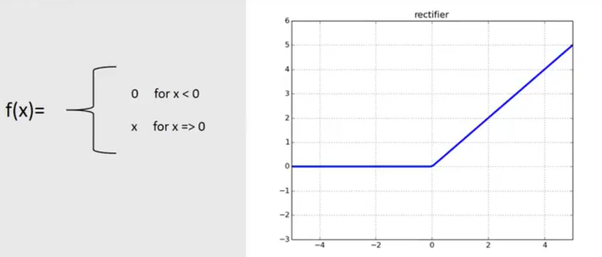
\includegraphics[width=0.7\linewidth]{Images/ReLUbreakdown}
	\caption{ReLU can be broken down into two linear units as shown in the figure for x $<$ 0 and x $\geq$ 0. This allows us to easily map the DNN equations in MILP models by breaking down the non-linearity inducing function.}
	\label{fig:relubreakdown}
\end{figure}

\section{Building the model}
\label{section:attacks}

As part of \tool, we provide automated attack synthesizers for the Artificial Pancreas System, Aircraft Collision Avoidance systems ACAS Xu and Horizontal CAS. 
As an example, we use a \ac{APS}.  
A \ac{APS} as shown in \label{fig:toyaps} consists of two sensor inputs that predict the amount of insulin as the output at some time $t$. 
\begin{figure}
	\centering
	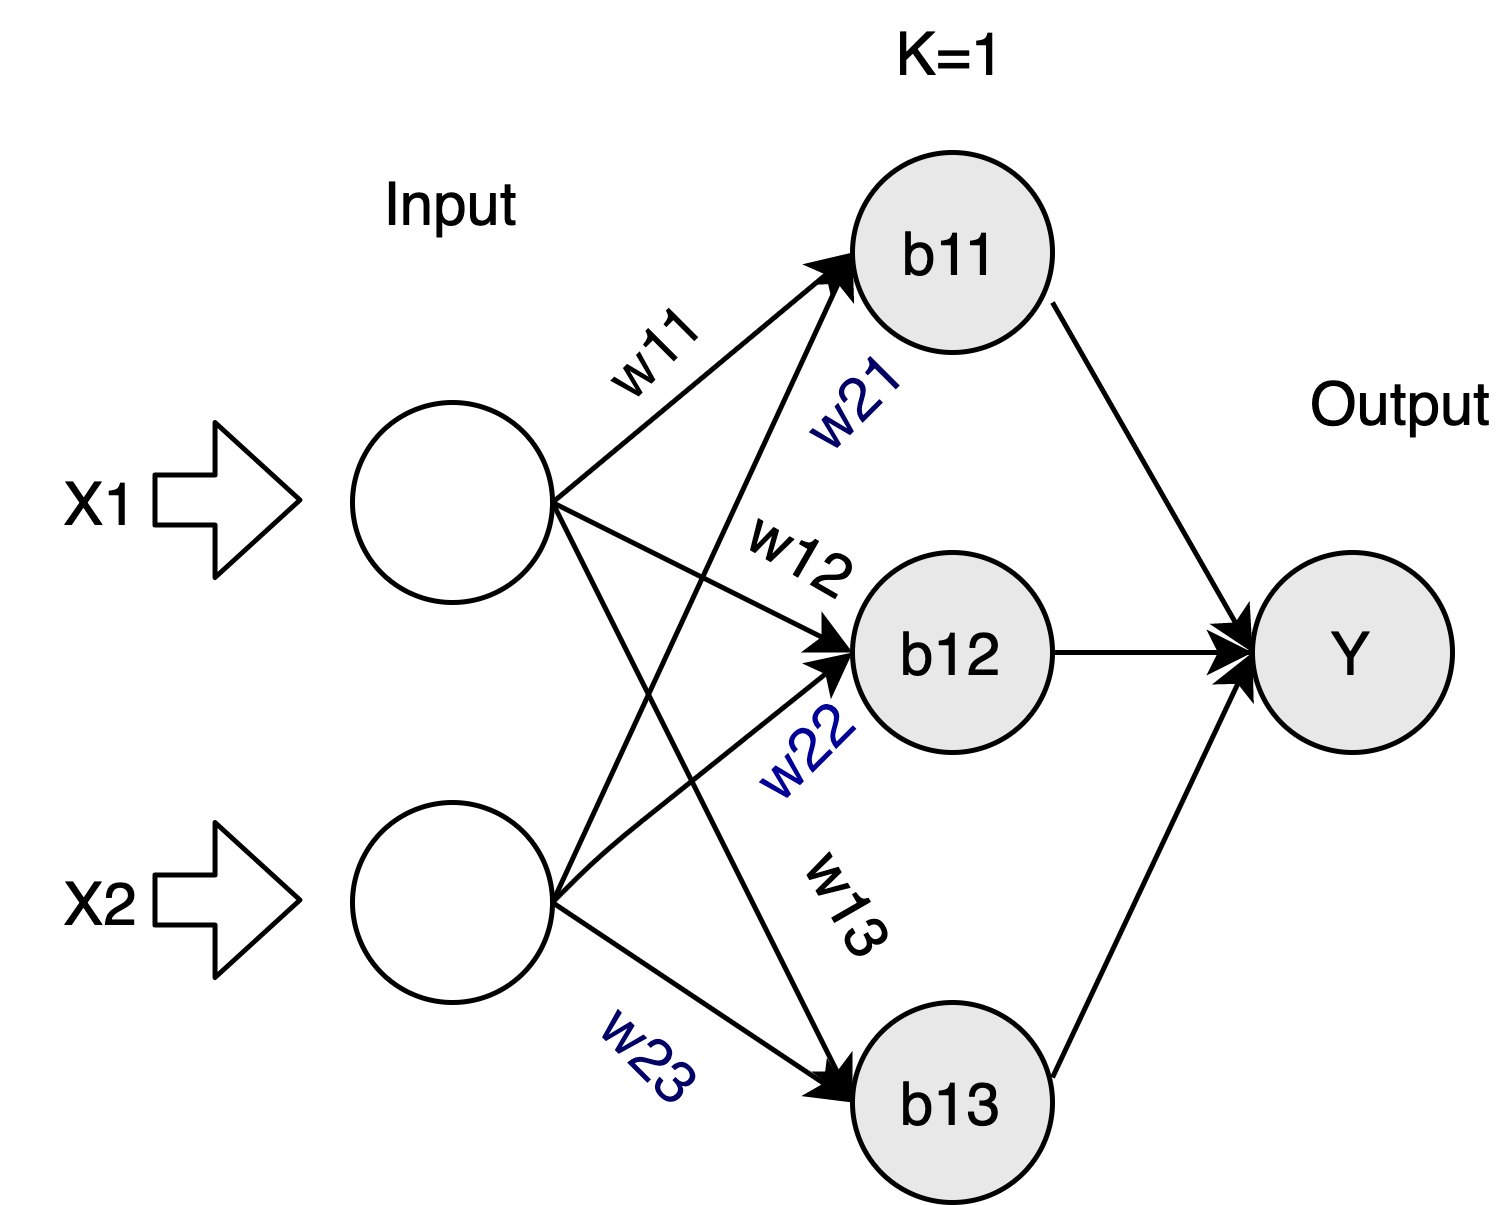
\includegraphics[width=0.7\linewidth]{Images/ToyAPS}
	\caption[APS]{APS that takes in two inputs which we consider as the sensor values from the human. It predicts the amount of insulin to be injected at some time based on the sensor inputs.}
	\label{fig:toyaps}
\end{figure}


\begin{algorithm}
	%\DontPrintSemicolon % Some LaTeX compilers require you to use \dontprintsemicolon    instead
	\KwIn{weight matrices, bias vectors, num\_layers, num\_neurons}
	\KwOut{DNN input, DNN output}
	Take the weight, bias, number of layers, and the number of neurons per layer. \\
	
	\textbf{Model}, \linebreak
	%\renewcommand{\labelenumi}{(\Roman{enumi})}
	%\begin{enumerate}[noitemsep,nolistsep]
	%\item
	(I) For every layer $k$ (with weight matrix $W_k$ and bias vector $b_k$), $output_k = W_k * input_k + b_k$
	\linebreak
	%\item 
	(II) Applying activation function to every layer's output,
	\linebreak
	Constraints: $ReLU\_output_k = max(0, output_k)$ (component-wise) \
	\linebreak
	The final layer's rectified output is the DNN output.
	
	\caption{Modeling neural network in MILP}
	\label{algo:b}
\end{algorithm}



The system can be represented as a MILP model through pseudo-code in Algorithm ~\ref{algo:b}. 
The model generated by this procedure is directly accepted by Gurobi (the solver we use for our experiments).
This converts the neural network structure into a set of linear equations that can be mapped directly into a back-end MILP solver.

An interesting point to note is that the DNN input is an output of Algorithm  ~\ref{algo:b}. 
This is because our procedure does not require an input to the DNN. 
This is because the resulting model can be solved to produce a valid input-output pair.
 Bounds can be enforced on the input variables by the user to ensure only
valid inputs are generated by the MILP solver. 
This is a positive consequence of using a constraint solving approach.
 The attacker does not need to have an input in hand when trying to compromise the system using \tool. 
 It also means that we can enumerate many such input-output pairs by repeatedly solving the model
and adding constraints to exclude previously seen solutions.

This is the general algorithm for converting any \ac{DNN} into a \ac{MILP} model. 
The difference in our evaluated systems and this system is only the difference between the number of layers and nodes in each layer that can be easily extended.
Our \tool  takes in a \ac{DNN} and automatically synthesizes \ac{MILP} models for it. 
Following the same algorithm we successfully synthesize models for \ac{APS}, \ac{ACAS-Xu}, and \ac{HCAS} within a minute. 

\begin{equation}
\label{10}
\begin{aligned}
x &= ReLU(w^Ty + b) \\
\end{aligned}
\end{equation}
Equation ~\ref{10} represents an \ac{APS}. 
We convert the equations above into a MILP model as shown in Algorithm ~\ref{algo:b}. 
Every layer is initially modeled as a linear equation. 
The activation function is represented as piecewise linear.
Our approach will work for any representation of a piece-wise linear function contingent to the fact that a non-linear function can be broken down into linear components.
Since we have abstracted away the details that represents non-linearity the future work would be representing non-linear functions as linear functions. 
 However, in our work, we focus on ReLU as explained in ~\ref{problemstatement}

\section{Modeling cost functions for attacks}
\label{section:costfunction}
%Why is modeling cost function important
Now that we have formulated the DNN as a MILP model, the next step is to add a cost or objective function to launch a specific kind of attack. 
This function allows the user to specify which inputs should be preferentially perturbed to generate a ripple.

In our \ac{APS}, we have two inputs $x_1$ and $x_2$ that map to an output $y$. 
To conduct \attack, the goal is to change the inputs in a way that the alarms are not triggered and yet it leads to an output change as we explained in Chapter ~\ref{attack}. 
These small changes lead the system to end up in a bad consequence eventually. 
In \ac{APS}, every small increase is a bad consequence of the system. 
Since the output determines the amount of insulin to be injected inside the body, small increases in the output.
Therefore, the attacker's goal is to change the output to $y'$, where $y' = y + a$. $a$ is some constant. 

%She needs to find the deviations in the input that would help her to change the outputs. 
However, the catch here is that the inputs perturbations should be very small such that the new input now provides her the output $y'$.  
The reason she wants the input perturbations to be small is that there are accompanying neural networks that determine the upper and lower bounds for inputs and outputs at every stage. 
The reason for these accompanying networks is to ensure the patients' safety as explained in Chapter ~\ref{attack}.


Algorithm ~\ref{algo:b} describes the process of modeling a neural network in a MILP format.
It does not consist of the cost function since the function will be different for different systems, depending on what the attacker wants to minimize and/or maximize.
In our case we are specifically demonstrating \ac{RFDIA}. 
The attackers model the objective function by introducing a new variable called $input\_delta$ . Hence, the equation ~\ref{1}.
in this section can be redefined as:

\begin{align}
\label{11}
y &=  ReLU(W(x + \bigtriangleup  x ) + b)\\
\end{align}

Algorithm ~\ref{algo:c} shows how to include the cost functions for \ac{RFDIA} as a part of the MILP model. 
 
\begin{algorithm}
	%\DontPrintSemicolon % Some LaTeX compilers require you to use \dontprintsemicolon    instead
	\KwIn{input ($x$), weight matrices, bias vectors, num\_layers, num\_neurons}
	\KwOut{input\_delta ($\Delta x$), layer\_output, ReLU\_output,}
	Take the weight, bias, number of layers and number of neurons per layer. \\
	
	\textbf{Model}, \linebreak
	%\renewcommand{\labelenumi}{(\Roman{enumi})}
	%\begin{enumerate}[noitemsep,nolistsep]
	%\item
	(I) For the first layer $k = 0$ (with weight matrix $W_0$ and bias vector $b_0$), $output_0 = W_0 * (x + \Delta x) + b_k$
	\linebreak
	(II) For every subsequent layer $k \geq 1$ (with weight matrix $W_k$ and bias vector $b_k$), $output_k = W_k * input_k + b_k$
	\linebreak
	%\item 
	(III) Applying activation function to every layer's output,
	\linebreak
	Constraints: $ReLU\_output_k = max(0, output_k)$ (component-wise) \
	\linebreak
	(IV) Applying constraints to the DNN output to force the desired deviation
	\linebreak
	The final layer's rectified output is the DNN output.
	
	\textbf{Cost/Attack Function} \linebreak
	$\min |\Delta x|$
	%$Minimize $  $input\_delta$
	\caption{Modeling neural network in MILP with perturbation variables and a cost function}
	\label{algo:c}
\end{algorithm}

If there are two inputs as in \ac{APS}, we can either try to minimize the delta values for both the inputs or only one of the inputs. 
The reason it is important to understand this is because, in general, within \ac{APS} there are inputs that come from two different sensors as explained in the motivating example section. 

The attacker might want to make changes to only one of the sensor readings. Hence, considering different scenarios, we can minimize the values depending on which inputs we are interested in targeting with an \ac{RFDIA}. 
The \ac{RFDIA} cost function in Algorithm ~\ref{algo:c} minimizes the absolute values of the perturbations to both inputs.
The solver can minimize the cost function despite it not being linear by introducing an extra variable for each input and adding two additional constraints per input that bound the input's value using this newly introduced variable. 
This would essentially linearize the cost function.


\section{Synthesizing attacks}
Once the attacker has a model and the cost function modeled, the next step is to identify the critical inputs and the desirable perturbations as explained in ~\ref{problemstatement}.
The attacker can run our obtained models along with the cost functions in our \ac{MILP} solver. 
In our running example of APS, in reality, there are 74 inputs collected from two sensors every five minutes.
 The goal of the attacker is to locate the critical inputs such that they can conduct \ac{RFDIA} at the right time.
 To do so, as described in the previous two sections, the approach implemented as \tool is used to chose the index of inputs to be perturbed.
 \tool allows us to set ranges using the methodology described above such that we can find the desirable perturbations. 
 

In this section we explain the intuition behind our approach and how we use the approach to model \tool. 
We further explain how we use \tool for synthesizing attacks from the models. 
In the next section we explain our results for three evaluation systems. 

